\documentclass[a4paper,12pt]{article}
\usepackage[utf8]{inputenc}
\usepackage[russian]{babel}
\usepackage{amsmath, amsfonts, amssymb}
\usepackage{geometry}
\usepackage{float}
\usepackage{booktabs}
\usepackage{multirow}
\usepackage{caption}
\usepackage{hyperref}
\usepackage{graphicx}

\usepackage{tikz}
\usetikzlibrary{automata, positioning, arrows.meta}

\usepackage{minted}
\usemintedstyle{colorful}

\geometry{left=2cm,right=2cm,top=2cm,bottom=2cm}
\hypersetup{colorlinks=true, linkcolor=black, urlcolor=blue}

\begin{document}
\begin{titlepage}
    \centering
    Федеральное государственное автономное образовательное учреждение высшего образования «Национальный исследовательский университет ИТМО» \\
    \vspace{1cm}
    Факультет Программной Инженерии и Компьютерной Техники \\
    \vfill
    {\large «Моделирование»} \\
    \vspace{0.5cm}
    Лабораторная работа №2 \\
    Марковские модели систем массового обслуживания \\
    Вариант N1 = 28 / N2 = 28 /  NG = 12
    \vfill
    \vspace{\fill}
    \begin{flushright}
        \textbf{Выполнили:} \\
        Козаченко Данил Александрович\\
        Яруков Артём Дмитриевич\\
        \textbf{Группа P3312} \\
        \textbf{Проверил:} \\
        Тропченко Андрей Александрович
    \end{flushright}
    \vspace{2cm}
    Санкт-Петербург
    2026г.
\end{titlepage}

\begin{centering}
    \renewcommand{\contentsname}{Содержание}
    \tableofcontents
\end{centering}
\newpage

\section{Цель работы}
Изучение метода марковских случайных процессов и его применение для исследования простейших моделей – систем массового обслуживания (СМО) с однородным потоком заявок.

\section{Постановка задачи и исходные данные}
Необходимо разработать, рассчитать и сравнить марковские модели двух систем массового обслуживания. Выбор наилучшего варианта построения СМО осуществляется в соответствии с заданным критерием.

\textbf{Критерий эффективности:} Сумма вариантов $N1+N2 = 28+28=56$ (четная), следовательно, критерий выбирается по варианту $N2=28$. Критерий «в» — \textbf{максимальная загрузка системы}.

\textbf{Параметры нагрузки (Вариант 12):}
\begin{itemize}
    \item Интенсивность входящего потока: $\lambda = 0.7$ (1/с);
    \item Средняя длительность обслуживания: $b = 5$ (с);
    \item Интенсивность обслуживания в приборе: $\mu = 1/b = 0.2$ (1/с);
    \item Вероятность направления заявки к прибору 1: $p_1 = 0.8$;
    \item Вероятность направления заявки к прибору 2: $p_2 = 0.05 + 0.15 = 0.2$.
\end{itemize}

\section{Описание исследуемых систем}
\textbf{СИСТЕМА\_1 (Вариант 28):}
Двухканальная гетерогенная СМО с раздельными накопителями. 
\begin{itemize}
    \item Число приборов: П = 2 ($\Pi_1, \Pi_2$).
    \item Емкости накопителей: $X=1$ (перед $\Pi_1$), $Y=2$ (перед $\Pi_2$).
    \item Заявка поступает с интенсивностью $\lambda = 0.7$. С вероятностью $p_1=0.8$ она направляется к $\Pi_1$ (интенсивность потока $\lambda_1 = 0.56$), с вероятностью $p_2=0.2$ — к $\Pi_2$ (интенсивность потока $\lambda_2 = 0.14$).
    \item Если накопитель выбранного прибора полон, заявка теряется.
\end{itemize}

\textbf{СИСТЕМА\_2 (Вариант 28):}
Одноканальная СМО с накопителем и неэкспоненциальным обслуживанием (модель $M/E_2/1/2$).
\begin{itemize}
    \item Число приборов: П = 1. Время обслуживания подчинено закону Эрланга 2-го порядка ($E_2$).
    \item Емкость накопителя (общая): ЕН = 2.
    \item Обслуживание представляется как прохождение заявкой двух экспоненциальных фаз (псевдосостояний), среднее время в каждой фазе $b/2 = 2.5$ с. Интенсивность перехода между фазами: $\mu_{ph} = 2\mu = 0.4$ (1/с).
\end{itemize}

\section{Перечень состояний марковского процесса}

\subsection{СИСТЕМА\_1}
Процессы в каналах протекают независимо. Состояние описывается вектором $(i, j)$, где $i \in \{0, 1, 2\}$ — число заявок в первой подсистеме (прибор + очередь 1), $j \in \{0, 1, 2, 3\}$ — число заявок во второй подсистеме (прибор + очередь 2). Всего 12 состояний.

Сопоставление номеров состояний в программе WinMark с физическими состояниями $(i, j)$:
\begin{itemize}
    \item $0 \to E_{0,0}$ (система пуста);
    \item $1 \to E_{1,0}$; \quad $2 \to E_{2,0}$;
    \item $3 \to E_{0,1}$; \quad $4 \to E_{1,1}$; \quad $5 \to E_{2,1}$;
    \item $6 \to E_{0,2}$; \quad $7 \to E_{1,2}$; \quad $8 \to E_{2,2}$;
    \item $9 \to E_{0,3}$; \quad $10 \to E_{1,3}$; \quad $11 \to E_{2,3}$.
\end{itemize}

\begin{figure}[H]
    \centering
    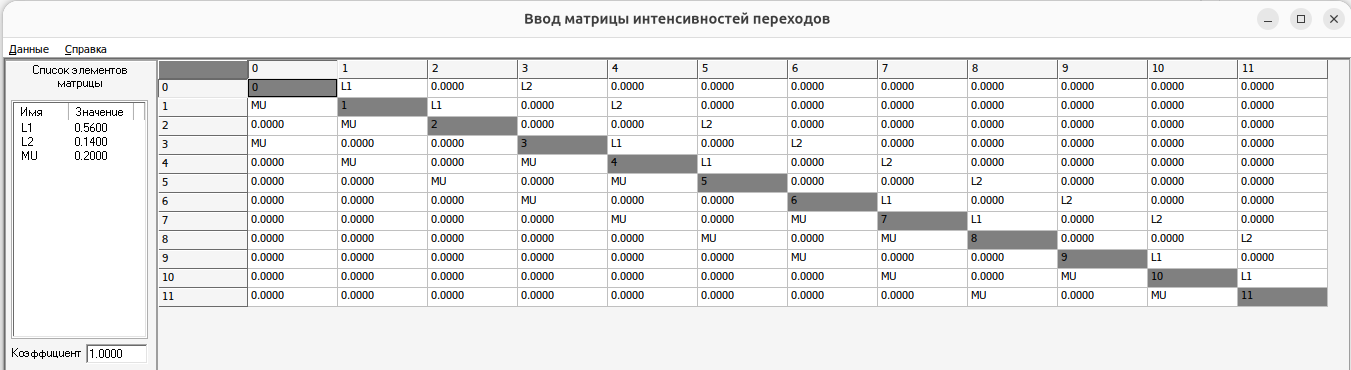
\includegraphics[width=1\linewidth]{matrix1.png}
    \caption{Матрица интенсивностей переходов СИСТЕМЫ\_1}
    \label{fig:matrix1}
\end{figure}

\subsection{СИСТЕМА\_2}
\begin{figure}[H]
    \centering
    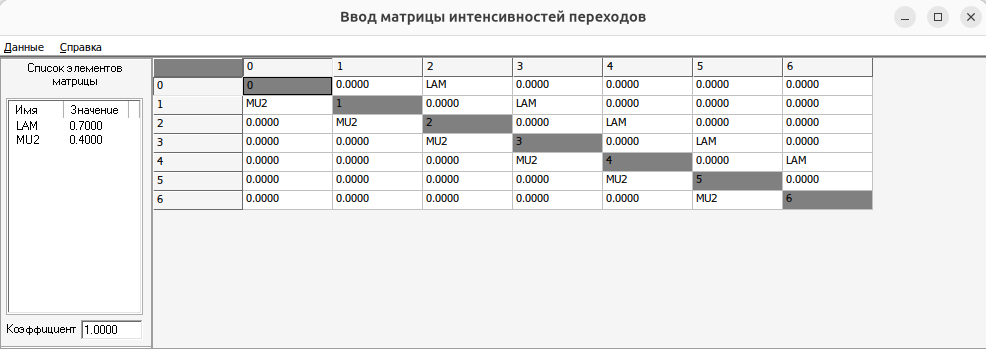
\includegraphics[width=1\linewidth]{matrix2.png}
    \caption{Матрица интенсивностей переходов СИСТЕМЫ\_2}
    \label{fig:matrix2}
\end{figure}
Применяется метод фиктивных фаз. Каждая заявка приносит в систему 2 фазы. Максимальное число заявок: 1 (в приборе) + 2 (в очереди) = 3. Максимальное число фаз в системе: $3 \times 2 = 6$.
Пусть $S_k$ — состояние, при котором в системе осталось выполнить $k$ фаз обслуживания:
\begin{itemize}
    \item $S_0$: система пуста (0 заявок, 0 фаз);
    \item $S_1, S_2$: 1 заявка в системе (на 2-й и 1-й фазе обслуживания соответственно);
    \item $S_3, S_4$: 2 заявки в системе (1 обслуживается, 1 в очереди);
    \item $S_5, S_6$: 3 заявки в системе (1 обслуживается, 2 в очереди — накопитель полон).
\end{itemize}
Всего 7 состояний. Приход заявки увеличивает индекс состояния на 2 (если есть место), завершение фазы уменьшает индекс на 1.

\section{Результаты работы}
\subsection{Размеченные графы переходов и матрицы}

\begin{figure}[H]
\centering
\begin{tikzpicture}[
    >=Stealth,
    state/.style={circle, draw, minimum size=1.0cm, inner sep=0pt, font=\small}
]
    % Координаты узлов (расстояние по X увеличено до 3.5 см, по Y до 2.5 см)
    % Строка 0 (j=0)
    \node[state] (00) at (0, 0) {$E_{0,0}$};
    \node[state] (10) at (3.5, 0) {$E_{1,0}$};
    \node[state] (20) at (7.0, 0) {$E_{2,0}$};

    % Строка 1 (j=1)
    \node[state] (01) at (0, -2.5) {$E_{0,1}$};
    \node[state] (11) at (3.5, -2.5) {$E_{1,1}$};
    \node[state] (21) at (7.0, -2.5) {$E_{2,1}$};

    % Строка 2 (j=2)
    \node[state] (02) at (0, -5.0) {$E_{0,2}$};
    \node[state] (12) at (3.5, -5.0) {$E_{1,2}$};
    \node[state] (22) at (7.0, -5.0) {$E_{2,2}$};

    % Строка 3 (j=3)
    \node[state] (03) at (0, -7.5) {$E_{0,3}$};
    \node[state] (13) at (3.5, -7.5) {$E_{1,3}$};
    \node[state] (23) at (7.0, -7.5) {$E_{2,3}$};

    % Горизонтальные переходы (Строка 0)
    \path[->] (00) edge [bend left=14] node[above] {\scriptsize $\lambda_1 = 0.56$} (10);
    \path[->] (10) edge [bend left=14] node[below] {\scriptsize $\mu = 0.2$} (00);
    \path[->] (10) edge [bend left=14] node[above] {\scriptsize $\lambda_1 = 0.56$} (20);
    \path[->] (20) edge [bend left=14] node[below] {\scriptsize $\mu = 0.2$} (10);

    % Горизонтальные переходы (Строка 1)
    \path[->] (01) edge [bend left=14] node[above] {\scriptsize $\lambda_1 = 0.56$} (11);
    \path[->] (11) edge [bend left=14] node[below] {\scriptsize $\mu = 0.2$} (01);
    \path[->] (11) edge [bend left=14] node[above] {\scriptsize $\lambda_1 = 0.56$} (21);
    \path[->] (21) edge [bend left=14] node[below] {\scriptsize $\mu = 0.2$} (11);

    % Горизонтальные переходы (Строка 2)
    \path[->] (02) edge [bend left=14] node[above] {\scriptsize $\lambda_1 = 0.56$} (12);
    \path[->] (12) edge [bend left=14] node[below] {\scriptsize $\mu = 0.2$} (02);
    \path[->] (12) edge [bend left=14] node[above] {\scriptsize $\lambda_1 = 0.56$} (22);
    \path[->] (22) edge [bend left=14] node[below] {\scriptsize $\mu = 0.2$} (12);

    % Горизонтальные переходы (Строка 3)
    \path[->] (03) edge [bend left=14] node[above] {\scriptsize $\lambda_1 = 0.56$} (13);
    \path[->] (13) edge [bend left=14] node[below] {\scriptsize $\mu = 0.2$} (03);
    \path[->] (13) edge [bend left=14] node[above] {\scriptsize $\lambda_1 = 0.56$} (23);
    \path[->] (23) edge [bend left=14] node[below] {\scriptsize $\mu = 0.2$} (13);

    % Вертикальные переходы (Колонка 0)
    \path[->] (00) edge [bend left=14] node[right=1pt] {\scriptsize $\lambda_2 = 0.14$} (01);
    \path[->] (01) edge [bend left=14] node[left=1pt] {\scriptsize $\mu = 0.2$} (00);
    \path[->] (01) edge [bend left=14] node[right=1pt] {\scriptsize $\lambda_2 = 0.14$} (02);
    \path[->] (02) edge [bend left=14] node[left=1pt] {\scriptsize $\mu = 0.2$} (01);
    \path[->] (02) edge [bend left=14] node[right=1pt] {\scriptsize $\lambda_2 = 0.14$} (03);
    \path[->] (03) edge [bend left=14] node[left=1pt] {\scriptsize $\mu = 0.2$} (02);

    % Вертикальные переходы (Колонка 1)
    \path[->] (10) edge [bend left=14] node[right=1pt] {\scriptsize $\lambda_2 = 0.14$} (11);
    \path[->] (11) edge [bend left=14] node[left=1pt] {\scriptsize $\mu = 0.2$} (10);
    \path[->] (11) edge [bend left=14] node[right=1pt] {\scriptsize $\lambda_2 = 0.14$} (12);
    \path[->] (12) edge [bend left=14] node[left=1pt] {\scriptsize $\mu = 0.2$} (11);
    \path[->] (12) edge [bend left=14] node[right=1pt] {\scriptsize $\lambda_2 = 0.14$} (13);
    \path[->] (13) edge [bend left=14] node[left=1pt] {\scriptsize $\mu = 0.2$} (12);

    % Вертикальные переходы (Колонка 2)
    \path[->] (20) edge [bend left=14] node[right=1pt] {\scriptsize $\lambda_2 = 0.14$} (21);
    \path[->] (21) edge [bend left=14] node[left=1pt] {\scriptsize $\mu = 0.2$} (20);
    \path[->] (21) edge [bend left=14] node[right=1pt] {\scriptsize $\lambda_2 = 0.14$} (22);
    \path[->] (22) edge [bend left=14] node[left=1pt] {\scriptsize $\mu = 0.2$} (21);
    \path[->] (22) edge [bend left=14] node[right=1pt] {\scriptsize $\lambda_2 = 0.14$} (23);
    \path[->] (23) edge [bend left=14] node[left=1pt] {\scriptsize $\mu = 0.2$} (22);
\end{tikzpicture}
\caption{Размеченный граф состояний и переходов СИСТЕМЫ\_1}
\label{fig:graph1}
\end{figure}

\begin{figure}[H]
\centering
\begin{tikzpicture}[
    >=Stealth, node distance=2.2cm, on grid, auto,
    state/.style={circle, draw, minimum size=0.8cm, font=\small}
]
    \node[state] (0) {$S_0$};
    \node[state] (1) [right=of 0] {$S_1$};
    \node[state] (2) [right=of 1] {$S_2$};
    \node[state] (3) [right=of 2] {$S_3$};
    \node[state] (4) [right=of 3] {$S_4$};
    \node[state] (5) [right=of 4] {$S_5$};
    \node[state] (6) [right=of 5] {$S_6$};

    % Переходы назад по обслуживанию (шаг 1)
    \path[->] (6) edge node[above=2pt] {\scriptsize $2\mu = 0.4$} (5);
    \path[->] (5) edge node[above=2pt] {\scriptsize $2\mu = 0.4$} (4);
    \path[->] (4) edge node[above=2pt] {\scriptsize $2\mu = 0.4$} (3);
    \path[->] (3) edge node[above=2pt] {\scriptsize $2\mu = 0.4$} (2);
    \path[->] (2) edge node[above=2pt] {\scriptsize $2\mu = 0.4$} (1);
    \path[->] (1) edge node[above=2pt] {\scriptsize $2\mu = 0.4$} (0);

    % Переходы вперед по приходу (прыжок через 2 состояния)
    \path[->] (0) edge [bend right=40] node[below=2pt] {\scriptsize $\lambda = 0.7$} (2);
    \path[->] (1) edge [bend right=40] node[below=2pt] {\scriptsize $\lambda = 0.7$} (3);
    \path[->] (2) edge [bend right=40] node[below=2pt] {\scriptsize $\lambda = 0.7$} (4);
    \path[->] (3) edge [bend right=40] node[below=2pt] {\scriptsize $\lambda = 0.7$} (5);
    \path[->] (4) edge [bend right=40] node[below=2pt] {\scriptsize $\lambda = 0.7$} (6);
\end{tikzpicture}
\caption{Размеченный граф состояний и переходов СИСТЕМЫ\_2}
\label{fig:graph2}
\end{figure}

\subsection{Стационарные вероятности (Форма 1)}

\begin{table}[H]
    \centering
    \caption{Стационарные вероятности состояний}
    \begin{tabular}{|c|c|c|c|c|}
        \hline
        \multirow{2}{*}{\textbf{Номер}} & \multicolumn{2}{c|}{\textbf{СИСТЕМА\_1}} & \multicolumn{2}{c|}{\textbf{СИСТЕМА\_2}} \\ \cline{2-5} 
         & \textbf{Обозначение} & \textbf{Вероятность} & \textbf{Обозначение} & \textbf{Вероятность} \\ \hline
        1 & $E_{0,0}$ & 0.0339 & $S_0$ & 0.0060 \\ \hline
        2 & $E_{1,0}$ & 0.0950 & $S_1$ & 0.0104 \\ \hline
        3 & $E_{0,1}$ & 0.0237 & $S_2$ & 0.0287 \\ \hline
        4 & $E_{2,0}$ & 0.2659 & $S_3$ & 0.0686 \\ \hline
        5 & $E_{1,1}$ & 0.0665 & $S_4$ & 0.1703 \\ \hline
        6 & $E_{0,2}$ & 0.0166 & $S_5$ & 0.4180 \\ \hline
        7 & $E_{2,1}$ & 0.1861 & $S_6$ & 0.2980 \\ \hline
        8 & $E_{1,2}$ & 0.0465 & - & - \\ \hline
        9 & $E_{0,3}$ & 0.0116 & - & - \\ \hline
        10& $E_{2,2}$ & 0.1303 & - & - \\ \hline
        11& $E_{1,3}$ & 0.0326 & - & - \\ \hline
        12& $E_{2,3}$ & 0.0912 & - & - \\ \hline
    \end{tabular}
\end{table}

\subsection{Характеристики систем (Форма 2)}

Расчет характеристик проводится непосредственно через стационарные вероятности состояний марковского процесса (как математическое ожидание дискретной случайной величины), а фундаментальные соотношения (формулы Литтла и баланса) используются для проверки полученных результатов.

\subsubsection*{1. СИСТЕМА\_1:}

\begin{itemize}
    \item \textbf{Нагрузка узлов и суммарная нагрузка:}
    \[
    y_1 = \lambda_1 b = 0.56 \cdot 5 = 2.8000, \quad y_2 = \lambda_2 b = 0.14 \cdot 5 = 0.7000
    \]
    \[
    Y = y_1 + y_2 = 2.8000 + 0.7000 = 3.5000.
    \]

    \item \textbf{Загрузка приборов (вероятность занятости):}
    \[
    \rho_1 = \sum_{i=1}^2 \sum_{j=0}^3 P_{i,j} = 1 - \sum_{j=0}^3 P_{0,j} = 1 - 0.0858 = 0.9142,
    \]
    \[
    \rho_2 = \sum_{i=0}^2 \sum_{j=1}^3 P_{i,j} = 1 - \sum_{i=0}^2 P_{i,0} = 1 - 0.3948 = 0.6052.
    \]
    Суммарная загрузка (среднее число занятых приборов):
    \[
    U_1 = \rho_1 + \rho_2 = 0.9142 + 0.6052 = 1.5194.
    \]
    Средний коэффициент занятости на один канал: $\rho_{\text{ср}} = \frac{U_1}{2} = 0.7597$.

    \item \textbf{Средняя длина очереди:}
    \[
    l_1 = 1 \cdot \sum_{j=0}^3 P_{2,j} = P_{2,0} + P_{2,1} + P_{2,2} + P_{2,3} = 0.6735,
    \]
    \[
    l_2 = 1 \cdot \sum_{i=0}^2 P_{i,2} + 2 \cdot \sum_{i=0}^2 P_{i,3} = 0.1934 + 2 \cdot 0.1354 = 0.4642.
    \]
    Суммарная длина очередей: $l = l_1 + l_2 = 0.6735 + 0.4642 = 1.1377$.

    \item \textbf{Среднее число заявок в подсистемах:}
    \[
    m_1 = \sum_{i=0}^2 i \cdot \left(\sum_{j=0}^3 P_{i,j}\right) = 1 \cdot 0.2406 + 2 \cdot 0.6735 = 1.5876,
    \]
    \[
    m_2 = \sum_{j=0}^3 j \cdot \left(\sum_{i=0}^2 P_{i,j}\right) = 1 \cdot 0.2763 + 2 \cdot 0.1934 + 3 \cdot 0.1354 = 1.0694.
    \]
    Суммарное число заявок в системе: $m = m_1 + m_2 = 1.5876 + 1.0694 = 2.6570$.
    
    \textit{Проверка баланса заявок:}
    \[
    m_1 = \rho_1 + l_1 = 0.9142 + 0.6735 = 1.5877 \approx 1.5876,
    \]
    \[
    m_2 = \rho_2 + l_2 = 0.6052 + 0.4642 = 1.0694 \quad (\text{совпадает}).
    \]

    \item \textbf{Вероятность потери заявок:}
    Заявка теряется, если соответствующий накопитель полон ($i=2$ для П1, $j=3$ для П2):
    \[
    \pi_1 = \sum_{j=0}^3 P_{2,j} = 0.6735, \quad \pi_2 = \sum_{i=0}^2 P_{i,3} = 0.1354.
    \]
    Суммарная вероятность потери по системе:
    \[
    \pi = p_1 \pi_1 + p_2 \pi_2 = 0.8 \cdot 0.6735 + 0.2 \cdot 0.1354 = 0.5388 + 0.0271 = 0.5659 \; (56.59\%).
    \]

    \item \textbf{Фактическая производительность:}
    \[
    \lambda_1' = \lambda_1(1 - \pi_1) = 0.56 \cdot (1 - 0.6735) = 0.1828 \text{ 1/с} \quad (\text{проверка: } \mu\rho_1 = 0.2 \cdot 0.9142 = 0.1828),
    \]
    \[
    \lambda_2' = \lambda_2(1 - \pi_2) = 0.14 \cdot (1 - 0.1354) = 0.1210 \text{ 1/с} \quad (\text{проверка: } \mu\rho_2 = 0.2 \cdot 0.6052 = 0.1210).
    \]
    Суммарная производительность: $\lambda' = \lambda_1' + \lambda_2' = 0.1828 + 0.1210 = 0.3038 \text{ 1/с}$.

    \item \textbf{Среднее время ожидания непосредственно по вероятностям состояний:}
Для канала П1 (заявка ожидает 1 период обслуживания $b$, если прибор занят и очередь пуста):
\[
w_1 = \frac{b \cdot \sum_{j=0}^3 P_{1,j}}{1 - \pi_1} = \frac{5 \cdot 0.2406}{1 - 0.6735} = 3.6845 \text{ с}.
\]
Для канала П2 (заявка ожидает 1 период $b$ при состоянии $j=1$ и 2 периода $2b$ при состоянии $j=2$):
\[
w_2 = \frac{b \cdot \sum_{i=0}^2 P_{i,1} + 2b \cdot \sum_{i=0}^2 P_{i,2}}{1 - \pi_2} = \frac{5 \cdot 0.2763 + 10 \cdot 0.1934}{1 - 0.1354} = 3.8347 \text{ с}.
\]
Среднее время ожидания по системе:
\[
w = \frac{\lambda_1' w_1 + \lambda_2' w_2}{\lambda'} = \frac{0.1828 \cdot 3.6845 + 0.1210 \cdot 3.8347}{0.3038} = 3.7445 \text{ с}.
\]
\textit{Проверка формулой Литтла:} $w_1 = \frac{l_1}{\lambda_1'} = \frac{0.6735}{0.1828} = 3.6844$ с, $w = \frac{l}{\lambda'} = \frac{1.1377}{0.3038} = 3.7449$ с (совпадает).
\end{itemize}

\subsubsection*{2. СИСТЕМА\_2:}

\begin{itemize}
    \item \textbf{Нагрузка системы:}
    \[
    y = \lambda b = 0.7 \cdot 5 = 3.5000.
    \]

    \item \textbf{Загрузка прибора:}
    \[
    \rho = \sum_{k=1}^6 P(S_k) = 1 - P(S_0) = 1 - 0.0060 = 0.9940.
    \]

    \item \textbf{Средняя длина очереди:}
    \[
    l = 1 \cdot (P(S_3) + P(S_4)) + 2 \cdot (P(S_5) + P(S_6)) = 1 \cdot 0.2389 + 2 \cdot 0.7160 = 1.6709.
    \]

    \item \textbf{Среднее число заявок в системе:}
    \[
    m = 1 \cdot (P(S_1) + P(S_2)) + 2 \cdot (P(S_3) + P(S_4)) + 3 \cdot (P(S_5) + P(S_6))
    \]
    \[
    m = 1 \cdot 0.0391 + 2 \cdot 0.2389 + 3 \cdot 0.7160 = 2.6649.
    \]
    \textit{Проверка баланса заявок:} $m = \rho + l = 0.9940 + 1.6709 = 2.6649$ (совпадает).

    \item \textbf{Вероятность потери заявок:}
    Заявка теряется, когда накопитель полон (состояния $S_5$ и $S_6$):
    \[
    \pi = P(S_5) + P(S_6) = 0.4180 + 0.2980 = 0.7160 \; (71.60\%).
    \]

    \item \textbf{Фактическая производительность:}
    \[
    \lambda' = \lambda(1 - \pi) = 0.7 \cdot (1 - 0.7160) = 0.1988 \text{ 1/с} \quad (\text{проверка: } \mu\rho = 0.2 \cdot 0.9940 = 0.1988).
    \]

    \item \textbf{Среднее время ожидания и пребывания непосредственно по вероятностям состояний:}

Заявка принимается системой в состояниях $S_0, S_1, S_2, S_3, S_4$. Условная вероятность застать систему в состоянии $S_k$ при условии приёма заявки равна $P(S_k) / (1 - \pi)$. Средняя длительность одной фазы обслуживания составляет $b_{\text{ph}} = b/2 = 2.5\text{ с}$.

Ожидание в очереди равно времени завершения всех $k$ фаз обслуживания, предшествующих поступившей заявке:
\[
w = \frac{\sum_{k=0}^{4} \left(k \cdot \frac{b}{2}\right) P(S_k)}{1 - \pi} = \frac{2.5 \cdot \big(0 \cdot P(S_0) + 1 \cdot P(S_1) + 2 \cdot P(S_2) + 3 \cdot P(S_3) + 4 \cdot P(S_4)\big)}{1 - 0.7160}
\]
\[
w = \frac{2.5 \cdot (0 + 0.0104 + 2 \cdot 0.0287 + 3 \cdot 0.0686 + 4 \cdot 0.1703)}{0.2840} = \frac{2.5 \cdot 0.9548}{0.2840} = \frac{2.3870}{0.2840} = 8.4049\text{ с.}
\]

Полное время пребывания складывается из времени ожидания и времени обслуживания собственной заявки ($2$ фазы со средним временем $b = 5\text{ с}$):
\[
u = \frac{\sum_{k=0}^{4} \left((k + 2) \cdot \frac{b}{2}\right) P(S_k)}{1 - \pi} = w + b = 8.4049 + 5.0 = 13.4049\text{ с.}
\]

\textbf{Проверка формулами Литтла:}
\[
w = \frac{l}{\lambda'} = \frac{1.6709}{0.1988} = 8.4049\text{ с,} \quad u = \frac{m}{\lambda'} = \frac{2.6649}{0.1988} = 13.4049\text{ с} \quad \text{(совпадает точно).}
\]
\end{itemize}

\begin{table}[H]
\centering
\caption{Характеристики систем (Форма 2)}
\label{tab:form2}
\small
\begin{tabular}{|l|c|c|c|c|}
\hline
\textbf{Характеристика} & \textbf{Прибор} & \textbf{Расчетная формула} & \textbf{СИСТ.1} & \textbf{СИСТ.2} \\ \hline
\multirow{3}{*}{Нагрузка ($y$)} 
 & П1 & $\lambda_1 b$ & 2.8000 & \multirow{3}{*}{3.5000} \\ \cline{2-4}
 & П2 & $\lambda_2 b$ & 0.7000 & \\ \cline{2-4}
 & Сумм. & $y_1 + y_2$ & 3.5000 & \\ \hline
\multirow{3}{*}{Загрузка ($\rho$)} 
 & П1 & $1 - \sum_{j=0}^3 P_{0,j}$ & 0.9142 & \multirow{3}{*}{0.9940} \\ \cline{2-4}
 & П2 & $1 - \sum_{i=0}^2 P_{i,0}$ & 0.6052 & \\ \cline{2-4}
 & Сумм. & $\rho_1 + \rho_2$ (для СИСТ.2: $1 - P(S_0)$) & 1.5194 & \\ \hline
\multirow{3}{*}{Длина очереди ($l$)} 
 & П1 & $\sum k \cdot P_{2,j}$ & 0.6735 & \multirow{3}{*}{1.6709} \\ \cline{2-4}
 & П2 & $\sum k \cdot P_{i,k+1}$ & 0.4642 & \\ \cline{2-4}
 & Сумм. & $l_1 + l_2$ & 1.1377 & \\ \hline
\multirow{3}{*}{Число заявок ($m$)} 
 & П1 & $\sum i \cdot P_{i,\cdot}$ & 1.5876 & \multirow{3}{*}{2.6649} \\ \cline{2-4}
 & П2 & $\sum j \cdot P_{\cdot,j}$ & 1.0694 & \\ \cline{2-4}
 & Сумм. & $m_1 + m_2$ & 2.6570 & \\ \hline
\multirow{3}{*}{\shortstack[l]{Время ожидания\\($w$), с}} 
 & П1 & $b \sum P_{1,j} / (1 - \pi_1)$ & 3.6845 & \multirow{3}{*}{8.4049} \\ \cline{2-4}
 & П2 & $(b \sum P_{i,1} + 2b \sum P_{i,2}) / (1 - \pi_2)$ & 3.8347 & \\ \cline{2-4}
 & Сумм. (ср.) & $(\lambda'_1 w_1 + \lambda'_2 w_2) / \lambda'$ & 3.7445 & \\ \hline
\multirow{3}{*}{\shortstack[l]{Время пребывания\\($u$), с}} 
 & П1 & $w_1 + b$ & 8.6845 & \multirow{3}{*}{13.4049} \\ \cline{2-4}
 & П2 & $w_2 + b$ & 8.8347 & \\ \cline{2-4}
 & Сумм. (ср.) & $w + b$ & 8.7445 & \\ \hline
\multirow{3}{*}{Вероятность потери ($\pi$)} 
 & П1 & $\sum_{j=0}^3 P_{2,j}$ & 0.6735 & \multirow{3}{*}{0.7160} \\ \cline{2-4}
 & П2 & $\sum_{i=0}^2 P_{i,3}$ & 0.1354 & \\ \cline{2-4}
 & Сумм. & $p_1 \pi_1 + p_2 \pi_2$ (для СИСТ.2: $P(S_5)+P(S_6)$) & 0.5659 & \\ \hline
\multirow{3}{*}{\shortstack[l]{Производительность\\($\lambda'$), 1/с}} 
 & П1 & $\lambda_1 (1 - \pi_1)$ & 0.1828 & \multirow{3}{*}{0.1988} \\ \cline{2-4}
 & П2 & $\lambda_2 (1 - \pi_2)$ & 0.1210 & \\ \cline{2-4}
 & Сумм. & $\lambda'_1 + \lambda'_2$ (для СИСТ.2: $\lambda(1 - \pi)$) & 0.3038 & \\ \hline
\end{tabular}
\end{table}

\subsection{Графики результатов варьирования}
\begin{figure}[H]
    \centering
    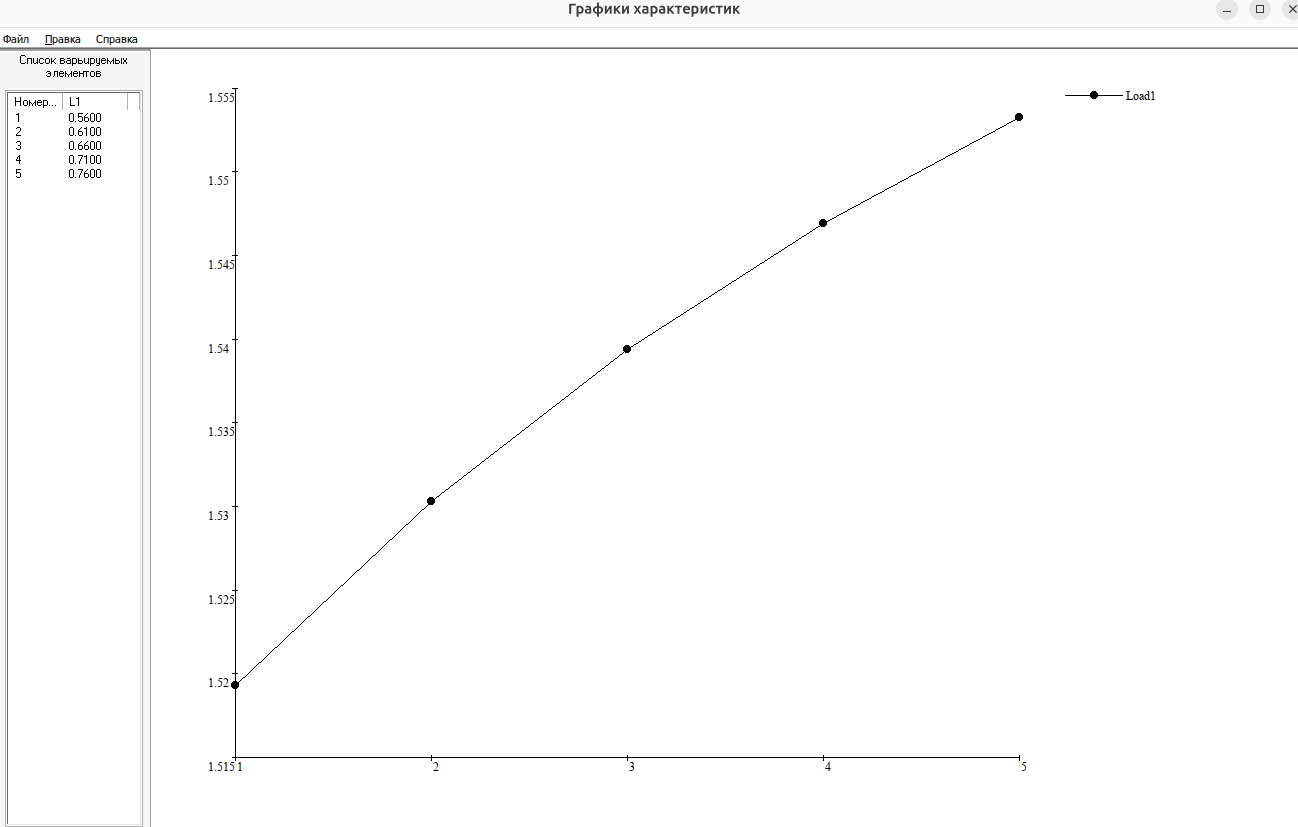
\includegraphics[width=\linewidth]{plot1.png}
    \caption{Зависимость загрузки $U_1$ от входного потока $L_1$ (СИСТЕМА\_1)}
    \label{fig:plot1}
\end{figure}
\begin{figure}[H]
    \centering
    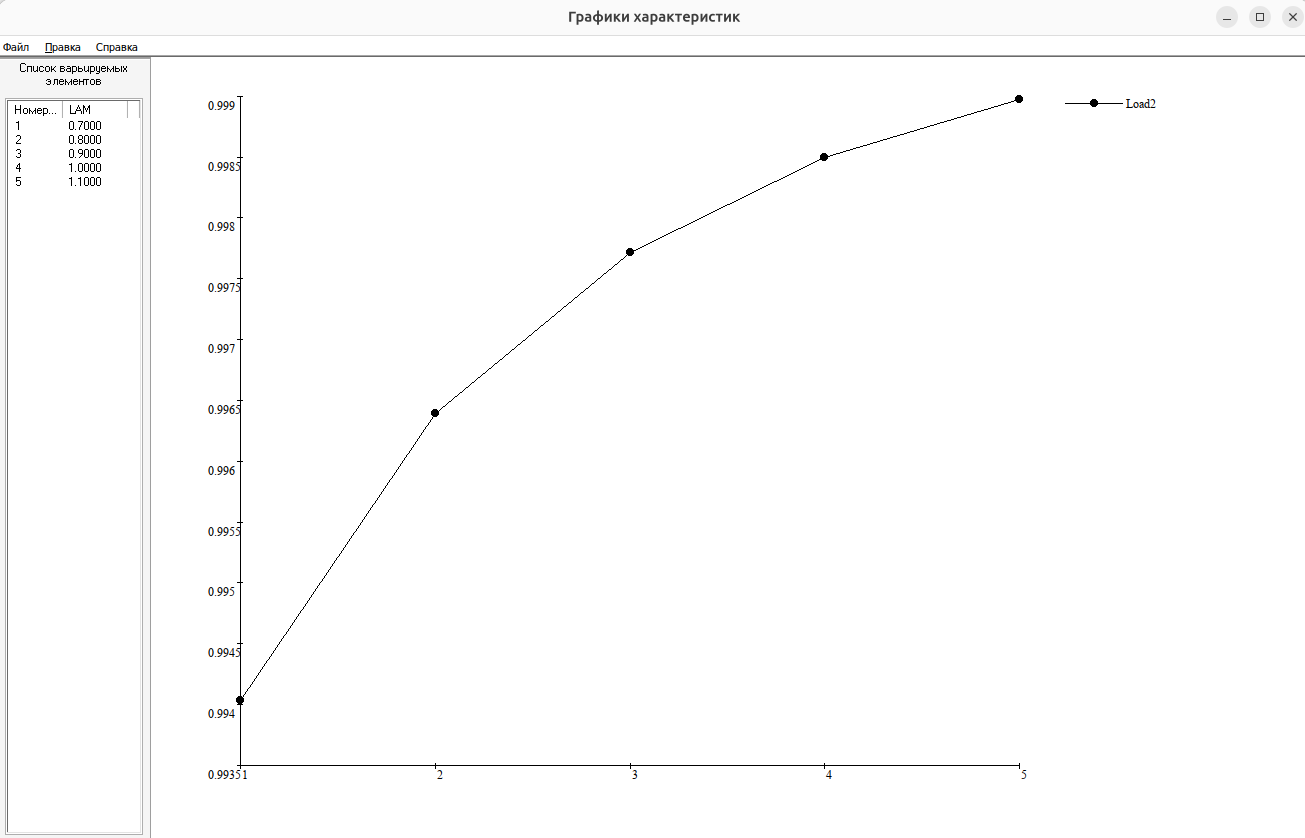
\includegraphics[width=\linewidth]{plot2.png}
    \caption{Зависимость загрузки $\rho$ от интенсивности входного потока $\lambda$ (СИСТЕМА\_2)}
    \label{fig:plot2}
\end{figure}

\textbf{Анализ результатов варьирования параметров:}
\begin{enumerate}
    \item \textbf{СИСТЕМА\_1 (Рис. 5):} При увеличении интенсивности потока к первому прибору от $L_1 = 0.56$ до $0.76$ (при неизменном $L_2 = 0.14$) суммарная загрузка системы $U_1$ монотонно возрастает от $1.519$ до $1.553$. Наличие двух независимых каналов обслуживания позволяет системе гибко реагировать на рост нагрузки: хотя первый прибор входит в режим глубокого насыщения ($\pi_1$ растет), второй канал продолжает стабильно функционировать с умеренной очередью.
    \item \textbf{СИСТЕМА\_2 (Рис. 6):} При варьировании входного потока $\lambda$ от $0.7$ до $1.1$ загрузка единственного прибора увеличивается крайне незначительно — от $0.9940$ до $0.9990$. Кривая асимптотически приближается к единице, что свидетельствует о практически полном насыщении обслуживающего прибора уже при базовой нагрузке. Весь дополнительный поток требований в такой системе приводит лишь к резкому росту вероятности отказа $\pi$ (свыше $75\%$), не увеличивая реальную пропускную способность.
\end{enumerate}

\section{Обоснование выбора наилучшего варианта}

В соответствии с заданным критерием эффективности --- \textbf{максимальная загрузка системы}:
\begin{itemize}
    \item \textbf{СИСТЕМА\_1:} представляет собой двухканальную систему. Суммарная загрузка оборудования (среднее число занятых обслуживанием приборов) составляет $U_1 = \rho_1 + \rho_2 = 1.5194$. При этом прибор 1 загружен на $91.42\%$, а прибор 2 --- на $60.52\%$. Средний коэффициент занятости оборудования составляет $\rho_{\text{ср}} = \frac{1.5194}{2} = 75.97\%$.
    \item \textbf{СИСТЕМА\_2:} является одноканальной системой с коэффициентом загрузки $\rho = 0.9940$ ($99.4\%$).
\end{itemize}

По показателю суммарного объема выполняемой работы (абсолютной загрузке) существенно превосходит первая система ($1.5194 > 0.9940$), поскольку в ней одновременно обслуживаются две заявки. Хотя формальный коэффициент занятости единственного прибора в СИСТЕМЕ\_2 выше ($99.4\%$ против средних $75.97\%$), это вызвано критической перегрузкой узла, приводящей к деградации качества обслуживания.

СИСТЕМА\_1 значительно превосходит СИСТЕМУ\_2 по всем функциональным характеристикам:
\begin{itemize}
    \item \textbf{Производительность:} выше в 1.53 раза ($0.3038$ против $0.1988$ 1/с);
    \item \textbf{Потери заявок:} ниже на 15 процентных пунктов ($56.59\%$ против $71.60\%$);
    \item \textbf{Средняя длина очереди:} меньше ($1.1377$ против $1.6709$ заявок);
    \item \textbf{Среднее время пребывания:} меньше в 1.53 раза ($8.745$ с против $13.405$ с).
\end{itemize}

Таким образом, конфигурация СИСТЕМЫ\_1 обеспечивает наивысшую фактическую загрузку оборудования полезной работой при существенно меньших потерях и задержках.

\section{Вывод}
По заданному критерию эффективности («максимальная загрузка системы») наилучшим вариантом является \textbf{СИСТЕМА\_1}. Двухканальная конфигурация с раздельными очередями обеспечивает более высокую суммарную занятость оборудования и лучшую пропускную способность по сравнению с одноканальной системой с эрланговским обслуживанием.
\end{document}